%% LyX 2.2.3 created this file.  For more info, see http://www.lyx.org/.
%% Do not edit unless you really know what you are doing.
\documentclass[11pt]{article}
\usepackage[latin9]{inputenc}
\usepackage{geometry}
\geometry{verbose}
\usepackage{amsmath}

\makeatletter
%%%%%%%%%%%%%%%%%%%%%%%%%%%%%% User specified LaTeX commands.


\usepackage{textcomp}
\usepackage{graphicx}
\usepackage{float}
% add other packages here

% put your group number and names in the author field
\title{\bf Exercise 2: A Reactive Agent for the Pickup and Delivery Problem}
\author{Group \textnumero 25: Goullet, Grondier	}

% the report should not be longer than 3 pages

\makeatother

\begin{document}
\maketitle

\section{Problem Representation}

\subsection{Representation Description}

% describe how you design the state representation, the possible actions, the reward table and the probability transition table

A state is represented by our class RLState: it has an obligatory
attribute describing the current city and two other optional describing
if it has a pickup task and the destination of the pickup task. There
are $N(N+1)$ possible states.

The possible actions is a mapping from each state to each possible
RLAction originating from the current city. There are $2N$ actions
originating from each city.

A reward is associated to each action as each action always has the
same reward. We get the reward for deliveries from Task Distribution,
and deduce the cost of traveling by knowing the distance between cities
and the cost per kilometer of moving.

The probability transition table is generated using the probability
of a pickup going for each city appearing at the destination city. 

\subsection{Implementation Details}

% describe the implementation details of the representations above and the implementation details of the reinforcement learning algorithm you implemented

\subsubsection{RLState}

RLState is our class representing a state. A state has a mandatory
$currentCity$ attribute. It also has a boolean attribute $hasTask$
to describe if the city has a task ready to be picked up, and am associated
destination city for the task $destinationCity$ . When building our
list of possible states, we ignore impossible actions, such as a task
with destination the source city.

\subsubsection{RLAction}

RLAction is our super-class representing an action. An action can
be a move (RLMove) or a pickup (RLPickup). We build an action list
corresponding to each state. Again, we ignore impossible actions or
actions refused by logist, such as moving to a non-neighbouring city,
the origin city, or delivering to the origin city.

\subsubsection{The Reward Table}

The reward table is a Map of the following form: $RLState \mapsto List(RLAction, Reward)$.

While iterating on our list of RLState, we create all RLAction possible
from this state, then we associate with it the reward. We substract
from the pickup reward the travel cost ($costPerKm*distance$), and
simple moves are just a net loss of the travel cost.

\subsubsection{The Probability Transition Table}

The probability transition table does not need to be built before
applying the algorithm: we can just deduce it from the probability
table given by the Task Distribution in the setup.

\section{Results}

% in this section, you describe several results from the experiments with your reactive agent

\subsection{Experiment 1: Discount factor}

% the purpose of this experiment is to understand how the discount factor influences the result

\subsubsection{Setting}

All figures have seed 42 and using the settings reactive.xml, but
we tested with other seeds. We tested with the following discount
values: 0, 0.5, 0.85, and 0.99.

\begin{figure}[H]
  \centering
  \begin{minipage}[b]{0.4\columnwidth}
    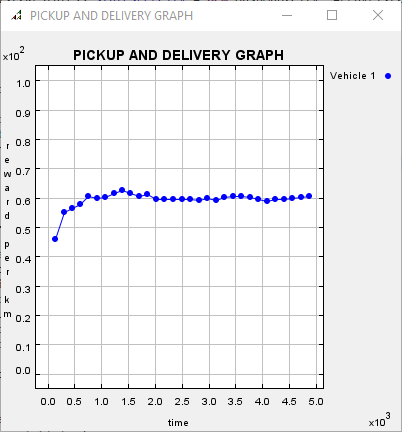
\includegraphics[width=\textwidth]{discount000.png}
    \caption{Discount = 0 \vspace{100px}}
  \end{minipage}
  \hfill
  \begin{minipage}[b]{0.4\columnwidth}
    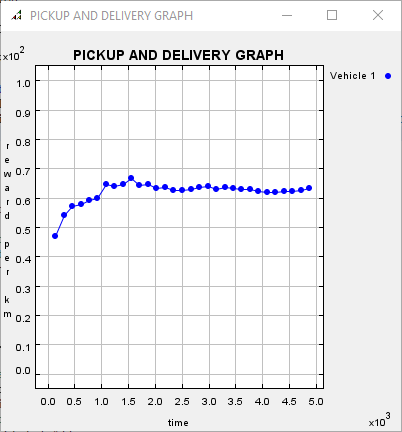
\includegraphics[width=\textwidth]{discount050.png}
    \caption{Discount = 0.5 }
  \end{minipage}
\end{figure} 
\begin{figure}[H]
  \begin{minipage}[b]{0.4\columnwidth}
    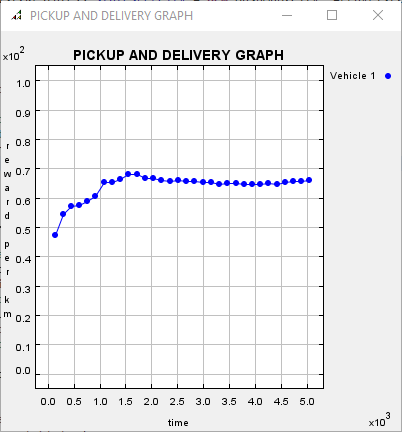
\includegraphics[width=\textwidth]{discount085.png}
    \caption{Discount = 0.85}
  \end{minipage}
  \hfill
  \begin{minipage}[b]{0.4\columnwidth}
    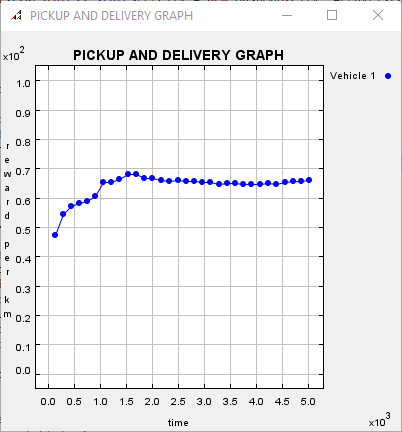
\includegraphics[width=\textwidth]{discount099.png}
    \caption{Discount = 0.99 }
  \end{minipage}
\end{figure}

% you describe how you perform the experiment (you also need to specify the configuration used for the experiment)

\subsubsection{Observations}

We observe as the Discount factor gets closer to 1, we usually get
better results. This is because when the discount factor gets closer
to 1, the number of iterations to calculate the most optimal decision
gets larger, and thus they are more precise. We also notice that there
is a diminishing return after a certain point, since we have reached
the ``good enough'' decision (In our example, 0.85 and 0.99). We
have tested with 0.999, and it takes roughly 10 times longer (14000
iterations vs 1000) to get only slightly better results.

\subsection{Experiment 2: Comparisons with dummy agents}

% you compare the results of your agent with two dummy agents: the random agent that was already given in the starter files and another dummy agent that you define and create. You should report the results from the simulations using the topologies given in the starter files and optionally, additional topologies that you create.

\subsubsection{Setting}

\begin{figure}[H]
  \centering
  \begin{minipage}[b]{0.4\columnwidth}
    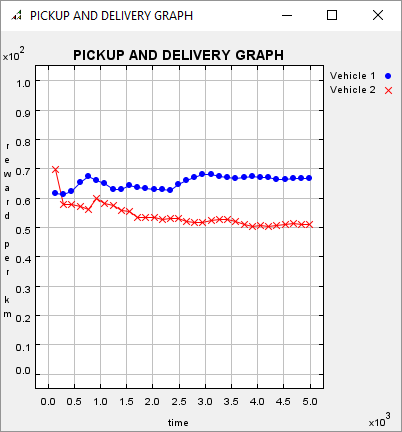
\includegraphics[width=\textwidth]{ddiscount085.png}
    \caption{Seed = 42. Discount = 0.85. RLAgent is Vehicle 1, Dummy agent is Vehicle 2}
  \end{minipage}
  \hfill
\end{figure} 

\subsubsection{Observations}

As we can see, our agent performs significantly better than a totally
random agent. We also notice that the graphs for the Reactive agent
isn't the same as previously because the addition of another agent
alters the task distribution. However in the end, our agent still
converges toward the same values.

\subsection{Experiment 3: Three of our agents}

% other experiments you would like to present

\subsubsection{Setting}

\begin{figure}[H]
  \centering
  \begin{minipage}[b]{0.4\columnwidth}
    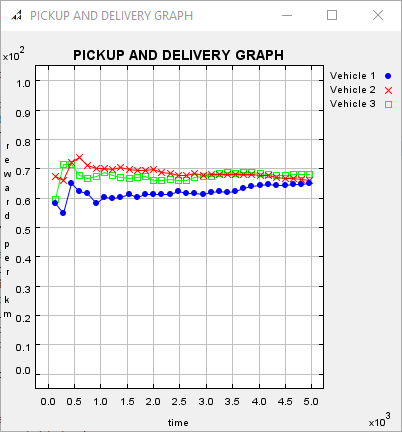
\includegraphics[width=\textwidth]{3agents.png}
    \caption{Seed = 42. Discount = 0.85}
  \end{minipage}
  \hfill
\end{figure} 

\subsubsection{Observations}

Even though each of the agents has different results at the begin,
they all end up converging toward the same value as found before.

\subsection{Experiment 3: Netherlands}

% other experiments you would like to present

\subsubsection{Setting}

\begin{figure}[H]
  \centering
  \begin{minipage}[b]{0.4\columnwidth}
    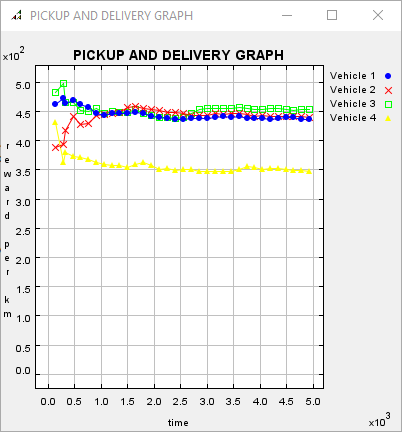
\includegraphics[width=\textwidth]{netherlands.png}
    \caption{Seed = 42. Discount = 0.85. All are RLA agents but vehicle 4.}
  \end{minipage}
  \hfill
\end{figure} 

\subsubsection{Observations}

There is nothing much to say that wasn't found in the previous analysis.
We would just like to not that closer cities with better connections
lead to better profits, even for a random agent.
\end{document}
